% Intended LaTeX compiler: pdflatex
\documentclass[../main]{subfiles}


\begin{document}

\section{Archivio TikZ}
\label{sec:orge039575}
\subsection{TikZ - Rete Neurale ReLU-feedforward}
\label{sec:orgbcb932a}
Rappresentazione di ``\href{20250624155858-neurone_artificiale.org}{Rete Neurale ReLU-feedforward}''

\begin{verbatim}
\documentclass[tikz,border=10pt]{standalone}
\usepackage{amsmath}
\usepackage{tikz}
\usetikzlibrary{decorations.pathreplacing, positioning}

\begin{document}

% Define variables for x positions of hidden layers
\def\Lone{1.5}
\def\Ltwo{3.0}
\def\Lthree{6.0}
\def\Lhidden{4.5}
\def\outputorizzontale{7.5}

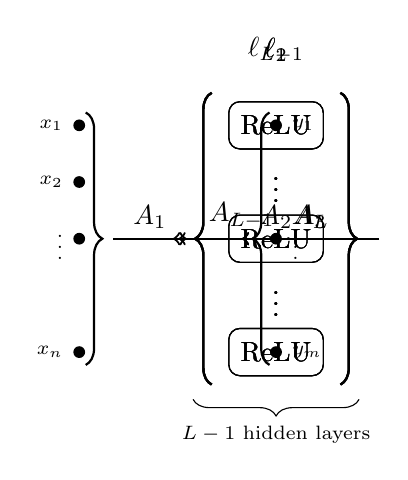
\begin{tikzpicture}[x=2.5cm, y=1.2cm,
    bullet/.style={circle, fill=black, inner sep=1.5pt},
    neuron/.style={rectangle, draw, rounded corners, minimum width=1.2cm, minimum height=6mm, inner sep=1pt},
    affine/.style={->, thick},
    brace/.style={decorate,decoration={brace,amplitude=6pt},thick},
    reverse brace/.style={decorate,decoration={brace,mirror,amplitude=6pt},thick},
    every label/.append style={font=\scriptsize}]

% Inputs (x1 to xn)
\node[bullet, label=left:$x_1$] (x1) at (0,1.2) {};
\node[bullet, label=left:$x_2$] (x2) at (0,0.6) {};
\node[bullet, label=left:$\vdots$] (xdots) at (0,0) {};
\node[bullet, label=left:$x_n$] (xn) at (0,-1.2) {};

% Brace grouping inputs
\draw[brace] ([xshift=4pt, yshift=3pt]x1.north west) -- ([xshift=4pt, yshift=-3pt]xn.south west);

% Hidden layer 1
\node at (\Lone,2.0) {$\ell_1$};
\node[neuron] (h11) at (\Lone,1.2) {ReLU};
\node at (\Lone,0.6) {$\vdots$};
\node[neuron] (h13) at (\Lone,0) {ReLU};
\node at (\Lone,-0.6) {$\vdots$};
\node[neuron] (h15) at (\Lone,-1.2) {ReLU};

\draw[brace] ([xshift=6pt,yshift=3pt]h11.north east) -- ([xshift=6pt,yshift=-3pt]h15.south east);
\draw[reverse brace] ([xshift=-6pt,yshift=3pt]h11.north west) -- ([xshift=-6pt,yshift=-3pt]h15.south west);

% A_1 arrow
\draw[affine] ([xshift=10pt]xdots.east) -- ([xshift=-15pt]h13.west) node[midway, above] {$A_1$};

% Hidden layer 2
\node at (\Ltwo,2.0) {$\ell_2$};
\node[neuron] (h21) at (\Ltwo,1.2) {ReLU};
\node at (\Ltwo,0.6) {$\vdots$};
\node[neuron] (h23) at (\Ltwo,0) {ReLU};
\node at (\Ltwo,-0.6) {$\vdots$};
\node[neuron] (h25) at (\Ltwo,-1.2) {ReLU};

\draw[brace] ([xshift=6pt,yshift=3pt]h21.north east) -- ([xshift=6pt,yshift=-3pt]h25.south east);
\draw[reverse brace] ([xshift=-6pt,yshift=3pt]h21.north west) -- ([xshift=-6pt,yshift=-3pt]h25.south west);

% A_2 arrow
\draw[affine] ([xshift=18pt]h13.east) -- ([xshift=-18pt]h23.west) node[midway, above] {$A_2$};

% Hidden layer L-1
\node at (\Lthree,2.0) {$\ell_{L-1}$};
\node[neuron] (hL1) at (\Lthree,1.2) {ReLU};
\node at (\Lthree,0.6) {$\vdots$};
\node[neuron] (hL3) at (\Lthree,0) {ReLU};
\node at (\Lthree,-0.6) {$\vdots$};
\node[neuron] (hL5) at (\Lthree,-1.2) {ReLU};

\draw[brace] ([xshift=6pt,yshift=3pt]hL1.north east) -- ([xshift=6pt,yshift=-3pt]hL5.south east);
\draw[reverse brace] ([xshift=-6pt,yshift=3pt]hL1.north west) -- ([xshift=-6pt,yshift=-3pt]hL5.south west);

% Other Hidden Layers

\node (Layerdots) at (\Lhidden,0) {$\dots$};

% A_{3} arrow
\draw[affine] ([xshift=20pt]h23.east) -- ([xshift=-3pt]Layerdots.west) node[midway, above] {$A_{3}$};

% A_{L-1} arrow
\draw[affine] ([xshift=3pt]Layerdots.east) -- ([xshift=-20pt]hL3.west) node[midway, above] {$A_{L-1}$};

% Final output layer
\node[bullet, label=right:$y_1$] (y1) at (\outputorizzontale,1.2) {};
\node[bullet, label=right:$\vdots$] (ydots) at (\outputorizzontale,0) {};
\node[bullet, label=right:$y_m$] (ym) at (\outputorizzontale,-1.2) {};

\draw[reverse brace] ([xshift=-4pt, yshift=3pt]y1.north east) -- ([xshift=-4pt, yshift=-3pt]ym.south east);

% Arrow to output
\draw[affine] ([xshift=20pt]hL3.east) -- ([xshift=-10pt]ydots.west) node[midway, above] {$A_{L}$};;


% Parentesi sotto
\draw[reverse brace, thin] ([xshift=-30pt]\Lone, -1.7) -- ([xshift=30pt]\Lthree, -1.7) node[midway, below, yshift=-6pt] {\scriptsize $L-1$ hidden layers};

\end{tikzpicture}

\end{document}
\end{verbatim}
\end{document}
